%%%%%%%%%%%%%%%%%%%%%%%%%%%%%%%%%%%%%%%%%%%%%%%%%%%%%%%%%%%%%%%%%%%%%%%%
%                                                                      %
%     File: Thesis_Results.tex                                         %
%     Tex Master: Thesis.tex                                           %
%                                                                      %
%     Author: Andre C. Marta                                           %
%     Last modified :  2 Jul 2015                                      %
%                                                                      %
%%%%%%%%%%%%%%%%%%%%%%%%%%%%%%%%%%%%%%%%%%%%%%%%%%%%%%%%%%%%%%%%%%%%%%%%

\chapter{V-F Optimization Mechanism}
\label{chapter:mech}


The results from the previous chapter display that the energy-efficiency (through the \acrshort{edp}) of an out-of-the-shelf \acrshort{gpu} can be significantly improved if a specific non-conventional V-F pair is applied on the Core \acrshort{dvfs} domain. 

However, in the previous chapter, one does not perform the frequency and voltage scaling dynamically, being one of the dissertation's objectives.
To address this dynamic tunning of frequency and voltage while using the increased exploration space (and taking into account that it is necessary to guarantee safe \acrshort{gpu} operation), two approaches can be followed: creating a forecasting model or creating an online optimization mechanism.

The forecasting model would predict the V-F pair to use based on the executing code (analysis of the Assembly code) and performance counters (the trace of the application being executed). This option has the benefit of allowing the complete execution of the target application under the best possible configuration. However, such a forecasting model would also have to take into consideration the \acrshort{gpu} temperature, utilization (the target application being executed by itself or concurrently with others) and more importantly, it would be very tied to a specific \acrshort{gpu} model. In so, this option would become complicated and not easily scalable between different \acrshort{gpu}s.

On the other hand, the online optimization mechanism can target the native code repetition on \acrshort{gpgpu} applications solving algorithms. For these applications, the best overall configuration is the best V-F pair for each algorithm's step. In algorithms where the time it takes to perform a step is significantly shorter than the time it takes to compute the total algorithm, it is possible to discover and achieve the optimal V-F configuration quickly. This approach has the added advantage of optimizing the \acrshort{gpu} for their current state: temperature, utilization, aging and all \acrshort{pvt} variation.

Due to the benefits of targeting the current \acrshort{gpu} state, the second approach, the creation of an online V-F optimization mechanism, is followed. 
Accordingly, this chapter is divided into two sections with the following outline: Section~\ref{section:opt} presents an overview  of the developed optimization mechanism, with its objective and requirements and Section~\ref{sec:usage} which presents how the users should use the developed mechanism to optimize their applications.



%%%%%%%%%%%%%%%%%%%%%%%%%%%%%%%%%%%%%%%%%%%%%%%%%%%%%%%%%%%%%%%%%%%%%%%%
\section{V-F Optimization Mechanism description}
\label{section:opt}

The devised V-F optimization mechanism is developed in Python and acts as a wrapper with functions that allow the user to implement the mechanism around its developing application. Figure~\ref{fig:layer} presents a layer diagram of the developed optimization mechanism, illustrating the main \acrshort{api}s used by the tool to communicate with the \acrshort{gpu} device, in order to control the voltage frequency pair that is applied on the \acrshort{dvfs} Core domain according to the user application output and device energy consumption and performance.

The user invokes the appropriate developed functions (more detail provided on Section~\ref{sec:usage}) that communicate with the gpowerSAMPLER, rocm-smi and ROCk \acrshort{api}s to retrieve and control the specific aspects of their \acrshort{gpu} device. The following subsections provide an in-depth explanation of each aspect of the mechanism.

\begin{figure}[htb]
  \centering
  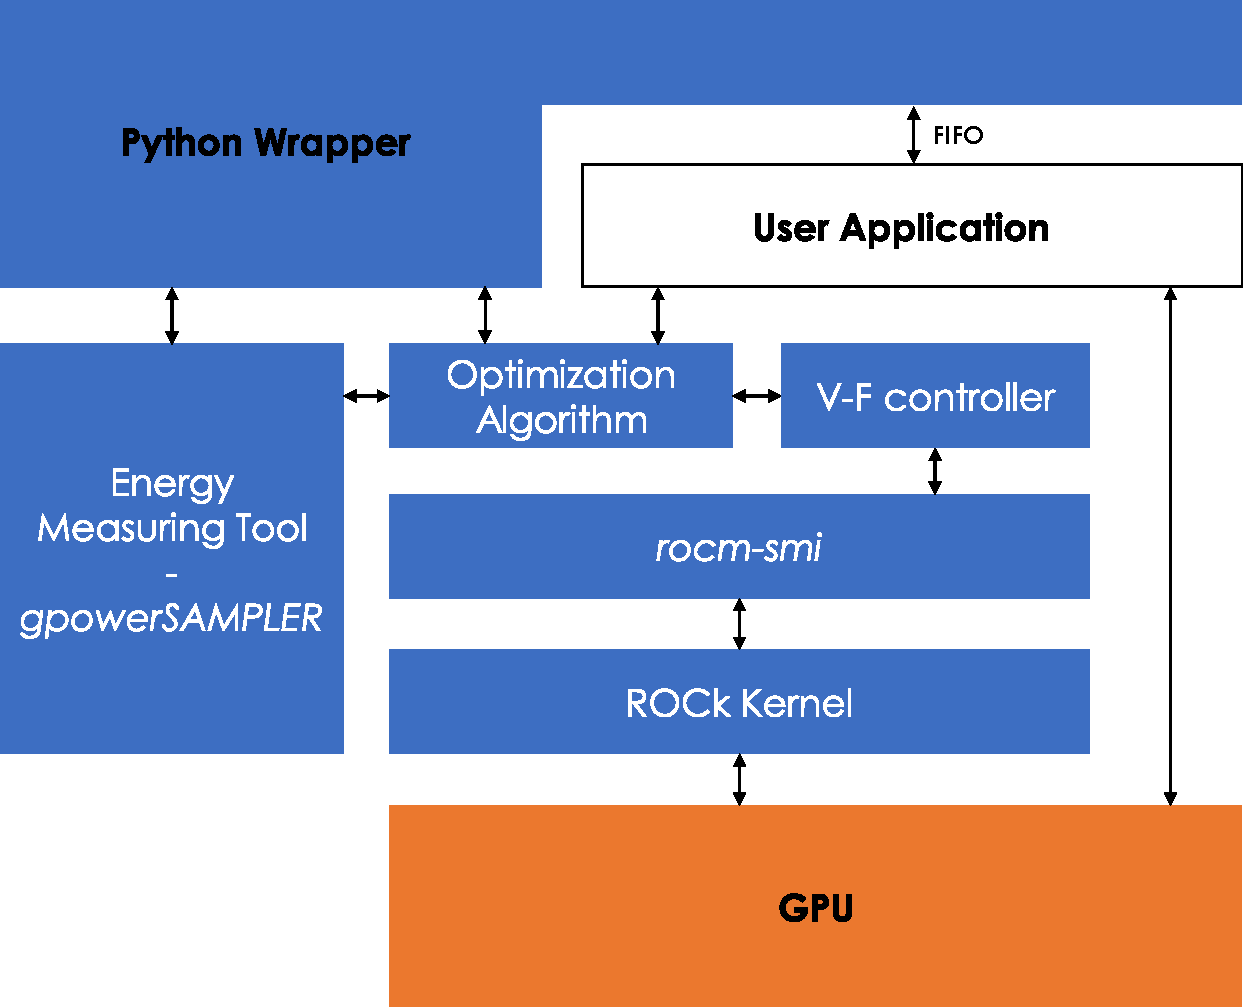
\includegraphics[width=0.6\textwidth]{Figures/Optimization/layerDiagram.pdf}
  \caption{Layer diagram of the developed V-F Optimization Mechanism.}
  \label{fig:layer}
\end{figure}



\subsection{Objective and Requirements}

The V-F optimization mechanism aims to discover and achieve the optimal V-F configuration to the running \acrshort{gpgpu} application and current \acrshort{gpu} state, optimizing for \textit{performance}, \textit{energy consumption} or \textit{energy-efficiency} (\acrshort{edp}). This optimal V-F configuration depends on the type of computations being performed, the \acrshort{gpu} temperature, utilization and aging and is selected from an exploration space concluded from the set of experiments covered on chapter~\ref{chapter:gpu_char}. 

The envisioned optimization mechanism is better suited to \acrshort{gpgpu} applications with a native code repetition - iterative algorithms like the training of deep neural networks. In particular, to applications where each iteration step takes significantly less time to compute than the algorithm's total computation time. This requirement is not mandatory; however, applications that follow this pattern can more significantly benefit from the mechanism since it can find the most appropriate configuration faster.

Another important characteristic of the optimization mechanism is that it takes into account the time that the regular \acrshort{gpu}s voltage frequency controllers take to change these parameters. As described in Chapter 2, the types of controllers that exist on out-of-the-shelf devices take between 200 to 500 ms to change and set the new V-F pair, making them not suitable to be continuously adapting to each and every operation being executed on the device. Instead, it is necessary to group a collection of operations (as described, a complete step of an algorithm) and find the most suitable V-F configuration for that set.
It is necessary to allow a portion of time between V-F changes to guarantee that the control mechanism has time to perform the change and stabilize both the frequency and the voltage before continuing to execute the computation.

As previously indicated, at the time of this dissertation, only AMD provides the necessary tools to independently control voltage and frequency, being that a requirement that is out of our control when designing this tool. However, if other manufacturers develop command-line applications that provide the same degree of control, this optimization mechanism can easily be ported to accommodate the same.


\subsection{Architecture Overview}


The devised V-F optimization mechanism follows the block diagram of Figure~\ref{fig:opt_mech}, consisting of a two-phase process where first data about the \acrshort{gpu} and application is gathered, and a second one where the algorithm is executed while the best V-F pair is found. 

\begin{figure}[htb]
  \centering
  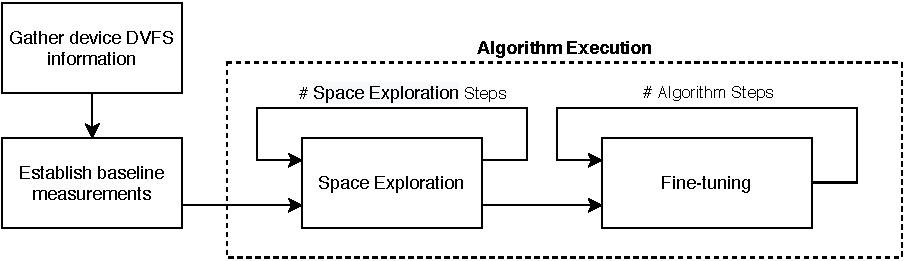
\includegraphics[width=0.95\textwidth]{Figures/Optimization/full_mech_5.pdf}
  \caption{V-F Optimization Mechanism Block Diagram.}
  \label{fig:opt_mech}
\end{figure}

On this context, the best V-F configuration is, depending on the optimization metric, the one that achieves the highest \textit{performance}, lowest \textit{energy consumption}, or higher \textit{energy efficiency} for the running application. Targeting the dissertation objective, the chosen and exemplified metric from now on is \textit{energy efficiency} compute as the \acrshort{edp}, where 
\begin{equation}
	EDP=energy * computation \: time.
	\label{eq:edp}
\end{equation}

\subsubsection{Gather DVFS information}

The proposed procedure starts with an initial stage where information about the current \acrshort{gpu} device \acrshort{dvfs} is gathered. This information is a summary of the characterization results obtained in Chapter 3, which includes the Core \acrshort{dvfs} default frequencies and voltages and attained $V_{min}$ of each frequency (that guaranteed correct operation in all tested benchmarks). The collected data sets the usable execution space (top right chart of Figure~\ref{fig:gpu_char}), which will be explored by the optimization mechanism.

\subsubsection{Establish baseline measurement}

In this stage, a step of the algorithm is executed with the highest frequency-voltage pair select, while the execution time and energy consumption are measured to compute the baseline \acrshort{edp} value. All the following measurements are normalized to this first result, in order to compare the results at different V-F pairs.


\subsubsection{Algorithm Execution}

In general, each stage of the Algorithm Execution phase follows the block diagram of Figure~\ref{fig:detail_mech}. Before executing the algorithm step, the energy and computation time measurement is started. After the step is concluded, the energy and computation time are computed, and in addition to specific application status, the results are provided for the optimization mechanism. 

\begin{figure}[htb]
  \centering
  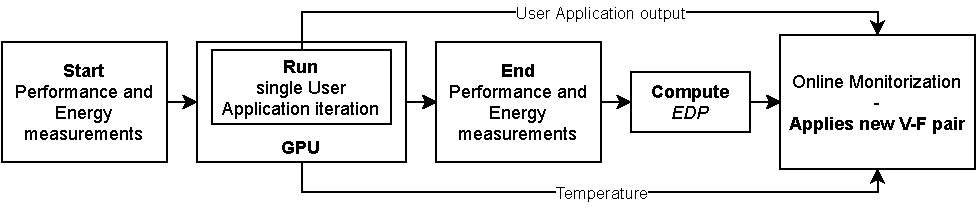
\includegraphics[width=0.75\textwidth]{Figures/Optimization/opt_pre_run.pdf}
  \caption{Pre-Run V-F Optimization Mechanism Block Diagram.}
  \label{fig:detail_mech}
\end{figure}

\subsubsection{Algorithm Execution - Space Exploration}

The objective of the this stage, \textit{Space Exploration}, is to find a V-F configuration that achieves an \acrshort{edp} value near the best possible one. In mathematical terms, to each V-F pair corresponds one \acrshort{edp} value, forming the function $EDP(f, V)$, so the objective is to find a good approximation of $min(EDP(f, V))$. The main difficulty is finding a valid configuration without testing all the possible ones, as performed on Chapter~\ref{chapter:gpu_char}. To tackle this problem, the mechanism applies the \textit{Simulated Annealing} algorithm to accept or reject a new V-F configuration based on the computed \acrshort{edp} value. This algorithm excels at finding an approximate global optimum in a fixed amount of iterations. 

At the end of each step of the space exploration stage, if the achieved \acrshort{edp} value is smaller than the current baseline, the current V-F configuration is stored alongside the \acrshort{edp} value as the current \textit{V-F pair baseline} and also inserted on a list of best configurations. If the tested configuration did not improve the \acrshort{edp} value, it can also be stored as \textit{V-F pair baseline} accordingly with the simulated annealing algorithm. Based on the current \textit{V-F pair baseline}, the new V-F configuration is randomly generated accordingly with Algorithm~\ref{alg:space-frequency} followed by Algorithm~\ref{alg:space-voltage}.

\begin{algorithm}
    \caption{Space Exploration - Generate new frequency.}
    \label{alg:space-frequency}
 \hspace*{\algorithmicindent} \textbf{Input:} $baseline\_frequency$: current baseline frequency \\
 \hspace*{\algorithmicindent} \textbf{Input:} $default\_frequencies$: list of available default frequencies \\
 \hspace*{\algorithmicindent} \textbf{Output:} $new\_frequency$: new random generated frequency
\begin{algorithmic}
\STATE $baseline\_frequency\_index \leftarrow$ get $baseline\_frequency$ index on $default\_frequencies$ list
\STATE $frequency\_step \leftarrow $choose random number from $\{-1, 0, 1\}$
\STATE $new\_frequency\_index \leftarrow baseline\_frequency\_index + frequency\_step$
\IF{$new\_frequency\_index < 0$}
\STATE $new\_frequency\_index \leftarrow 0$
\ELSIF{$new\_frequency\_index >$ length($default\_frequencies$) $-1$}
\STATE $new\_frequency\_index \leftarrow$ length($default\_frequencies$) $-1$
\ENDIF
\STATE $new\_frequency \leftarrow default\_frequencies[new\_frequency\_index]$
\end{algorithmic}
\end{algorithm}

\begin{algorithm}
\caption{Space Exploration - Generate new voltage.}
    \label{alg:space-voltage} 
    \hspace*{\algorithmicindent} \textbf{Input:} $baseline\_voltage$: current baseline voltage \\
 \hspace*{\algorithmicindent} \textbf{Input:} $new\_frequency$: new random generated frequency \\
 \hspace*{\algorithmicindent} \textbf{Input:} $UES(f)$: usable exploration space, provides the maximum and minimum voltage for a given frequency \\
 \hspace*{\algorithmicindent} \textbf{Output:} $new\_voltage$: new random generated voltage
\begin{algorithmic}
\STATE $voltage\_step \leftarrow $choose random number from $\{-50, -25,0, 25, 50\}$
\STATE $new\_voltage \leftarrow baseline\_voltage + voltage\_step$
\IF{$new\_voltage < UES(new\_frequency)[minimum]$}
\STATE $new\_voltage \leftarrow$ minimum voltage of usable execution space for $new\_frequency$
\ELSIF{$new\_voltage < UES(new\_frequency)[maximum]$}
\STATE $new\_voltage \leftarrow$ maximum voltage of usable execution space for $new\_frequency$
\ENDIF
\end{algorithmic}
\end{algorithm}


If, after $ N $ execution steps, if no better configuration is found, or the predefined \textit{Space Exploration Steps} are concluded, the \textit{Space Exploration} phase is ended, and the list of best configurations is analyzed, with the V-F configuration that achieved the best \acrshort{edp} acting as a baseline for the \textit{Fine-Tuning} phase.


\subsubsection{Algorithm Execution - Fine-tuning}

After the execution of the \textit{Space Exploration} phase, a quasi-optimal configuration is found. The second phase is responsible for fine-tuning the V-F pair obtained by the previous stage to achieve the actual global minimum of $EDP(f, V)$. That optimal configuration may be between two default frequencies and at a voltage level than required to discretize the voltage range more finely.

The overall scheme of this phase is similar to the \textit{Space Exploration}. However, in this case, the \textit{Hill Climbing} algorithm is used instead. This algorithm only accepts a new configuration if it is able to further minimize the \acrshort{edp} value, being specialized in finding the global optimization minimum having the certainty that it is on the neighborhood of the initial phase V-F configuration. The new V-F configuration is now obtained with Algorithm~\ref{alg:fine-frequency} followed by Algorithm~\ref{alg:fine-voltage}.

\begin{algorithm}
    \caption{Fine-tuning - Generate new frequency.}
    \label{alg:fine-frequency}
 \hspace*{\algorithmicindent} \textbf{Input:} $baseline\_frequency$: current baseline frequency \\
 \hspace*{\algorithmicindent} \textbf{Input:} $default\_frequency\_range$: minimum and maximum available frequencies \\
 \hspace*{\algorithmicindent} \textbf{Output:} $new\_frequency$: new random generated frequency
\begin{algorithmic}
\STATE $frequency\_step \leftarrow $choose random number from $\{-10, 0, 10\}$
\STATE $new\_frequency\ \leftarrow baseline\_frequency + frequency\_step$
\IF{$new\_frequency < default\_frequency\_range[minimum]$}
\STATE $new\_frequency \leftarrow default\_frequency\_range[minimum]$
\ELSIF{$new\_frequency > default\_frequency\_range[maximum]$}
\STATE $new\_frequency \leftarrow default\_frequency_range[maximum]$
\ENDIF
\end{algorithmic}
\end{algorithm}

\begin{algorithm}
\caption{Fine-tuning - Generate new voltage.}
    \label{alg:fine-voltage} 
    \hspace*{\algorithmicindent} \textbf{Input:} $baseline\_voltage$: current baseline voltage \\
 \hspace*{\algorithmicindent} \textbf{Input:} $new\_frequency$: new random generated frequency \\
 \hspace*{\algorithmicindent} \textbf{Input:} $UES(f)$: usable exploration space, provides the maximum and minimum voltage for a given frequency \\
 \hspace*{\algorithmicindent} \textbf{Output:} $new\_voltage$: new random generated voltage
\begin{algorithmic}
\STATE $voltage\_step \leftarrow $choose random number from $\{-10,0, 10\}$
\STATE $new\_voltage \leftarrow baseline\_voltage + voltage\_step$
\STATE $pair\_default\_frequencies \leftarrow $ compute pair of frequencies around $new\_frequency$
\STATE $minimum\_voltage(f) \leftarrow$ compute a linear interpolation between\\ 
\hspace*{\algorithmicindent}$UES(pair\_default\_frequencies[inferior])[minimum]$ and\\
\hspace*{\algorithmicindent}$UES(pair\_default\_frequencies[inferior])[minimum]$
\STATE $maximum\_voltage(f) \leftarrow$ compute a linear interpolation between\\
\hspace*{\algorithmicindent}$UES(pair\_default\_frequencies[inferior])[maximum]$ and\\
\hspace*{\algorithmicindent}$UES(pair\_default\_frequencies[inferior])[maximum]$
\IF{$new\_voltage < minimum\_voltage(new\_frequency)$}
\STATE $new\_voltage \leftarrow minimum\_voltage(new\_frequency)$
\ELSIF{$new\_voltage < maximum\_voltage(new\_frequency)$}
\STATE $new\_voltage \leftarrow maximum\_voltage(new\_frequency)$
\ENDIF
\end{algorithmic}
\end{algorithm}



\subsection{Online Monitorization}

The online monitorization is in action on the algorithm executions phases of the optimization mechanism. It introduces two other inputs to the optimization mechanism, device temperature and application status that help to guarantee that the system is safe to use. These two new metrics impact the amount of undervoltage allowed, by changing the voltage produced by Algorithms~\ref{alg:space-frequency} to \ref{alg:fine-voltage}. As depicted in Figure~\ref{fig:monitorization}, the Algorithms~ref{alg:space-frequency} generates a new V-F pair based on the current baseline V-F configuration. The new configuration is then provided to the \textit{Analyze Application Output} procedure that receives a flag from the user that indicates if the last application output is valid (for example, a float did not become a Not a Number - NaN). If that is the case, this block increases the voltage by $10$mV. Finally, the chosen frequency is given to the \textit{Temperature Model} depicted in Section~\ref{sec:temp_model}, which reduces the amount of undervoltage when the device temperature surpasses the 70ºC.  At the end of these three stages, the new V-F pair is generated and applied on the \acrshort{gpu} in order for the algorithm execution to proceed.

\begin{figure}[htb]
  \centering
  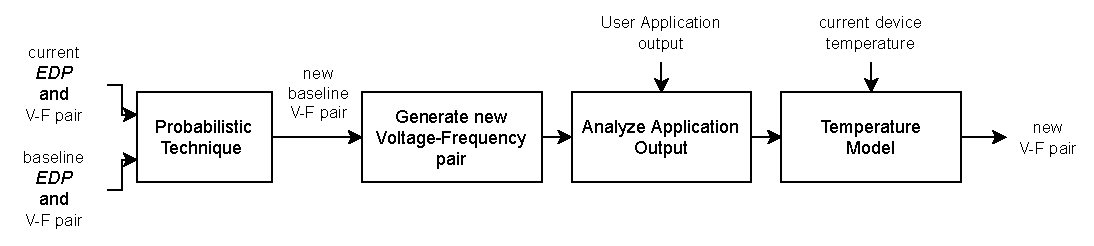
\includegraphics[width=0.9\textwidth]{Figures/Optimization/online_monitoring.pdf}
  \caption{Online Monitorization Block Diagram.}
  \label{fig:monitorization}
\end{figure}



To note that the analyze of the application output acts as a fail-safe that should not be necessary if a valid exploration space and temperature model are acquired for the present \acrshort{gpu}.



\section{Users guide}
\label{sec:usage}

This section presents the correct way for users to include the V-F optimization mechanism on their \acrshort{gpgpu} applications. As indicated, the wrapper that provides all the functions to enable this mechanism was developed in Python. Using this languange, it is possible to launch any other application developed in Python or not. To accomodate those cases, the interface between the Python wrapper and the user application is made through a named pipe (FIFO).

Listing~\ref{lst:wrapper} provides an example of the order and place where each function call should be performed and where the user should insert its application code.


\begin{figure}[h]
    \begin{lstlisting}[language=Python, caption=Example of usage of V-F Optimization Mechanism, label=lst:wrapper, basicstyle=\footnotesize\ttfamily,abovecaptionskip=0pt, captionpos=b]
    initOptimizationMechanism(pathToCharacterizationResults)
    ...
    initMesurements()
    ... execute baseline execution ...
    baselineMeasurements = computeMesurements()
    ...
    for epoch in range(space_exploration_epochs):
        initMesurements()
        
        ... code of application step ...
        
        measurements = computeMesurements()
        
        outputValid = analiseOutput(output)
        
        # analyses the measurements, application output, temperature
        # generates and applies new V-F configuration
        optimizationMechanismSpaceExploration(measurements, outputValid)
    ...
    for epoch in range(total_number_of_epochs - space_exploration_epochs):
        initMesurements()
        
        ... code of application step ...
        
        measurements = computeMesurements()
        
        outputValid = analiseOutput(output)
        
        # analyses the measurements, application output, temperature
        # generates and applies new V-F configuration
        optimizationMechanismFineTunning(measurements, outputValid)
    ...
    \end{lstlisting}
\end{figure}


The user should implement the \texttt{analiseOutput()} function in accordance with Listing~\ref{lst:analiseOutput}

\begin{figure}[h]
    \begin{lstlisting}[language=Python, caption=analiseOutput function prototype, label=lst:analiseOutput, basicstyle=\footnotesize\ttfamily,abovecaptionskip=0pt, captionpos=b]
    def analiseOutput(output):
        ... analise output variable content to understand if output is valid ...
        if(valid)
            return True
        return False
    \end{lstlisting}
\end{figure}

\section{Summary}

The development of the V-F Optimization Mechanism described in this chapter fulfills the objective of having a concrete manner of providing a non-conventional \acrshort{dvfs} system. The devised mechanism uses the previous chapter's experimental results to enable a final user to use the uncover V-F pairs to extract better energy-efficiency of their devices without having any detailed knowledge of the \acrshort{gpu} architecture.

The following chapter provides the application of both the characterization and implementation of this mechanism to improve the energy-efficiency of the Vega 10 \acrshort{gpu} when running deep learning applications.